\section{Methodology}\label{sec:METHOD}

We focus this paper on the fact, that information, sufficient for classification, is stored in dataset items, located close to the class border. 

We also limit our experiments with few important assumptions. Firstly, we mostly discuss binary classification cases. Secondly, we address the idea that dataset has a property of a metric space, and with a high probability nearest neighbours (in terms of the metric) of the item belong to the same class as the item. This sometimes referred as \emph{compactness hypothesis} \cite{compactness}.

Core idea lays in the fact that for dense enough proximity graphs, \emph{graph cut} can be used for a robust approximation of the class boundaries. Here we understand graph cut as a \emph{set of edges, where source and destination vertices belong to different classes}. We utilize this idea in two ways: discrete and continuous. Graph cut is visualized in figure ~\ref{fig:cut}.

\begin{figure}
    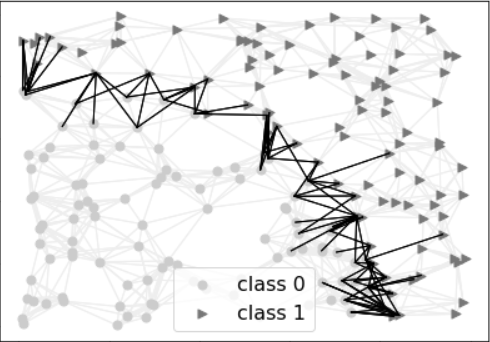
\includegraphics[width=3.3in]{paper/images/00_cut.png}
    \caption{Black edges represent graph cut. They have source and destination nodes in different classes.}
    \label{fig:cut}
\end{figure}

\subsection{Discrete case}

Following the compactness hypothesis, we can say, that if we know exact location of class boundaries, for classification we can generalize idea of ray casting algorithm for point in polygon problem. If we also know which class is at which side of the border, we need only the last border crossing to answer the question about the class of the item. Also, we don't actually need straight ray: any continuous path through metric space will be enough to detect the fact of crossing the border. In proximity graphs, namely NSW/HNSW we can obtain such a path by greedily traversing the edges towards the classifier vector, which result in near-shortest path, estimated as $\mathbb{E}(log(|V|)$. Here is the simple algorithm ~\ref{alg:the_alg} that reflects the idea.

\begin{algorithm}
\label{alg:the_alg}
\SetAlgoLined
\KwResult{class label}
 $v \gets$ random vertex from $V$ of NSW\;
 $d_{new} \gets distance(v, destination)$\;
 $class_{new} \gets v.class$\;
 \Repeat{$d_{new} > d$}{
  $d \gets d_{new}$\;
  $class \gets class_{new}$\;
  $v \gets closest(v.neighbours, destination)$\;
  $d_{new} \gets distance(v, destination)$\;
  $class_{new} \gets v.class$\;
 }
 \KwRet{$class$}\;
 \caption{Greedy path casting algorithm in NSW for multiclass classification}
\end{algorithm}

We implement this idea as an improvement to the exact implementation of NSW paper repository, and compared speed and accuracy of classification to original 1-NN classification accuracy on the few problems, including synthetic multidimensional data, handwritten digits dataset \cite{mnist} storing 1797 64-dimensional vectors, 100 leaves dataset with 1600 64-dimensional vectors \cite{100leaves} and road signs dataset \cite{signsdataset} with 43 classes (images were resized to 256-dimesional representation).


\subsection{Continuous case}

In continuous case we want to extremely reduce dataset size while still being able to classify new items accurately. We put an assumption, that classifier function is defined as $f:\mathbb{R}^D \rightarrow [0, 1]$ where $0$ and $1$ correspond to confident class attribution. We also assume that the classifier is a differentiable function $f\in\mathbb{C}_1$.
Now we can use compactness hypothesis to propose the idea, that for an ideal classifier gradient of $f$ is 0 almost everywhere, except class border neighbourhood: $\nabla f = 0$. We also know, that proximity graph cut is a discrete representation of a class border. Thus, we can build a function $g(x|cut):\mathbb{R}^D\rightarrow\mathbb{R}^D$, which interpolates graph cut to represent gradient of classifier function $\nabla f \approx g$.

We propose to use weighted averaging of $\epsilon$-neighbour-hood for interpolation method to build $g$, where $\epsilon$ is taken as median shortest distance between edge centers multiplied by hyperparameter $R$. We store edges in a NSW index for faster neighbourhood retrieval. Results are presented on figure ~\ref{fig:gradfield}. You can check details of implementation in \texttt{modules/nsw/cut\_classifier.py} file in our repository. We also tried different radial basis functions for interpolation, but could not achieve good results at low-dimensional cases. As we are interested in a fast and robust computation method, we address this problem in our future studies and discuss this in section ~\ref{sec:DISCUSSION}.

\begin{figure}
    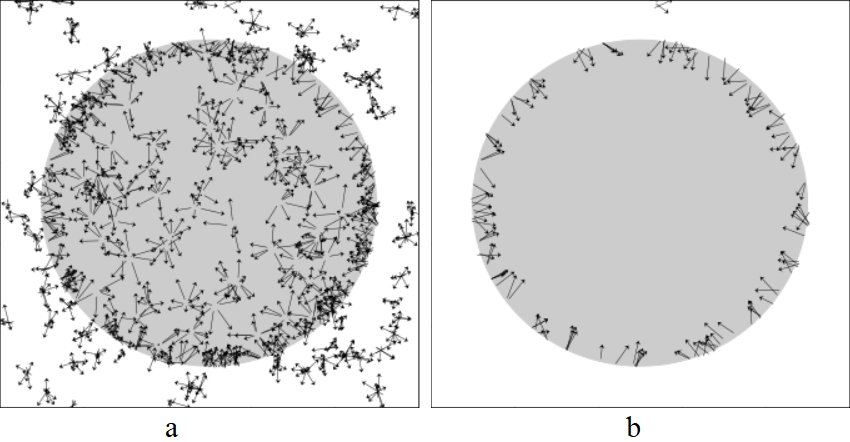
\includegraphics[width=3.3in]{paper/images/01_grad_field.png}
    \caption{Gradient field approximation based on graph cut. Dark area corresponds to class 1. (a) based on graph raw data (b) after Wilson-like editing.}
    \label{fig:gradfield}
\end{figure}

As $g(\mathbf{x})$ is an analytical function, good idea would be restoring an approximate classifier function $\hat{f}$  given it's gradient $g$. Unfortunately there is no common solution for multidimensional cases \cite{fieldbygrad}. Another difficulty is that we cannot guarantee that $\Rot g=0$ which is required for a gradient of function $\hat{f}$.

To solve this problem with integration we propose to combine ray casting method with Gradient theorem \cite{gradth}, which state that ${\displaystyle \int_{\gamma}\nabla f (\mathbf {r} )\cdot \mathrm {d} \mathbf {r} =f\left(\mathbf {x} \right)-f \left(\mathbf {a} \right)}$, where $\gamma$ correspond to arbitrary path between $\mathbf{a}$ and $\mathbf{x}$. We propose to use approximate discrete version of this formula ~\ref{eqn:graddiscrete}.

\begin{equation}
\label{eqn:graddiscrete}
\hat{f}(\mathbf{x}) \approx \hat{f}(\mathbf{a}) + \sum_{i=1}^{N}g\left(\mathbf{a}+\frac{i(\mathbf{x}-\mathbf{a})}{N}\right) \cdot \frac{(\mathbf{x}-\mathbf{a})}{N}
\end{equation}

if we know exact class value for some vector $\mathbf{a}$, we can cast a straight ray $(\mathbf{x}-\mathbf{a})$ directly to vector of interest $\mathbf{x}$. Thus, we uniformly subsample small set of reference vectors $support$ together with their classes. By assumption the size of the set is less of equal to 10\% of the original dataset. We store these vectors in NSW index for faster neighbourhood retrieval. If there is a class border, integration will give us the value with the sign same to $\mathbf{x}.class - \mathbf{a}.class$. If there is no border, integration part will be approximately $0$. We use $small$ hyperparameter to threshold $0$. If $x$ is located in a class border neighbourhood, few reference points can be used for voting, which is managed by a hyperparameter. Proposed idea is described in pseudocode algorithms ~\ref{alg:integral}.

\begin{algorithm}
\label{alg:integral}
\SetAlgoLined
\KwResult{class label}
 $a \gets$ closest vertex to $x$ from index $support$\;
 $class \gets a.class$\;
 $r \gets x - a$\;
 $G \gets 0$\;
 \For{$i\gets1$ \KwTo $N$}{
    $G \gets G + g\left(a + \frac{i*r}{N}\right)\cdot r$\;
 }
 $G \gets \frac{G}{N}$\;
 \If{$|G|>threshold$}{
    $class \gets 1 - class$
 }
 \KwRet{$class$}\;
 \caption{Ray casting algorithm for classification}
\end{algorithm}

Proposed idea is neat in theory, but when facing real data can fail. We discovered a problem with mislabelled samples. Each such sample in a graph creates an incoming or outgoing cut, which forms a "bump" or a "hole" in $\hat{f}(x)$ respectively. These function fluctuations dramatically drop classification accuracy especially in high dimensional cases.

To overcome this difficulty we implement adaptation of Wilson editing \cite{Wilson}. Originally this procedure requires removal of items which are mislabelled according to kNN classification. This both remove outliers and smoothes class border. We replace kNN classification with adjacent nodes voting. If a node belongs to graph cut, we examine it for being an "island" or "peninsula": we reject all nodes together with edges, if majority of neighbours fall into other class. We implement this idea in algorithm~\ref{alg:wilsoncut}. Constant $\frac{3}{2}$ appears from NSW recommendations to have $3*D$ edges per node. Thus, we test that the node has at least one half adjacent nodes from the other class.

\begin{algorithm}
\label{alg:wilsoncut}
\SetAlgoLined
 $Cut \gets$ graph cut\;
 $Threshold \gets \frac{3}{2}*$ (data dimensions)\;
 \For{$node$ in $Cut$}{

    $Flow \gets$ $\{e \in Cut | node \in e \}$\;
    \If{$|Flow| > Threshold$}{
            $Cut \gets Cut \setminus Flow$\;
    }
 }
 \caption{Wilson-like graph cut editing algorithm}
\end{algorithm}

To sum up, continuous case is a generalization of kNN voting, where vote computation is done in a different form. Instead on using actual nearest neighbours, we use closest vectors from a small $support$ set and test if there is a class border between these vectors and assessed vector $\textbf{x}$. Example of restored classifier function is presented at figure ~\ref{fig:clfimg}.

\begin{figure}
    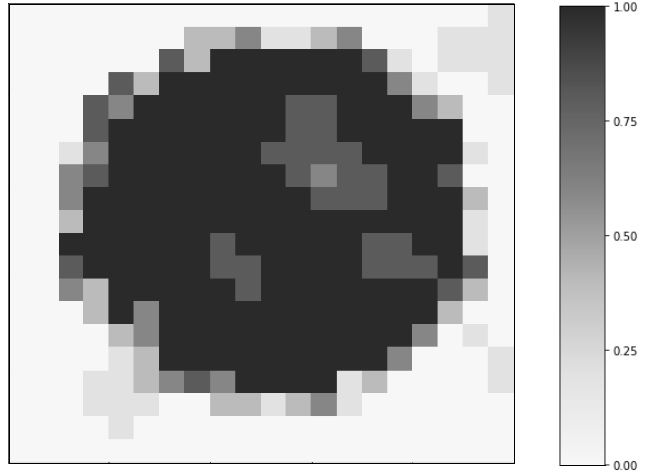
\includegraphics[width=0.5\textwidth]{paper/images/03_clf_grad.png}
    \caption{Restored classifier function using gradient method.}
    \label{fig:clfimg}
\end{figure}